\documentclass[../Main.tex]{subfiles}

\begin{document}
    
% przed tym chapterem przydałoby się opisać transfer stylu, rozwój prac od 2015
% do 2018, funkcję straty dla transferu stylu, jej interpretację, na czym polega
% AdaIn (https://arxiv.org/abs/1703.06868), czemu była całkeim okej ale nie do końca.
% Takie jej ograniczenia, które ta praca, na której bazujemy rozwiązuje
\subsection{Neural Network}
    In this chapter we describe the neural network used for style transfer. 
    First we describe it's architecture and specific layers. Then we detail
    pruning procedure used to obtain the final model.
    \subsubsection{Overall network architecture} 
    We follow architecture described in \cite{Li2018}, changing it's components' details 
    in order to enable real time inference. The network consists of two 
    main components - encoder-decoder module and
    transformation module pictured in Figure \ref{fig:overall_network}.
    To perform style transfer encoder is fed with content image
    and style image, producing feature maps cF and sF respectively.
    Next, transformation module transfers sF's statistics onto cF. Resulting 
    feature map is passed through decoder, which creates final image. 
    Thanks to this modular architecture, each style image needs to be encoded
    only once. For both encoder-decoder and
    transformation module we use pretrained models publicly available at 
    \url{https://github.com/sunshineatnoon/LinearStyleTransfer}
    as starting point for further development. 
    
    \begin{figure}[h!]
        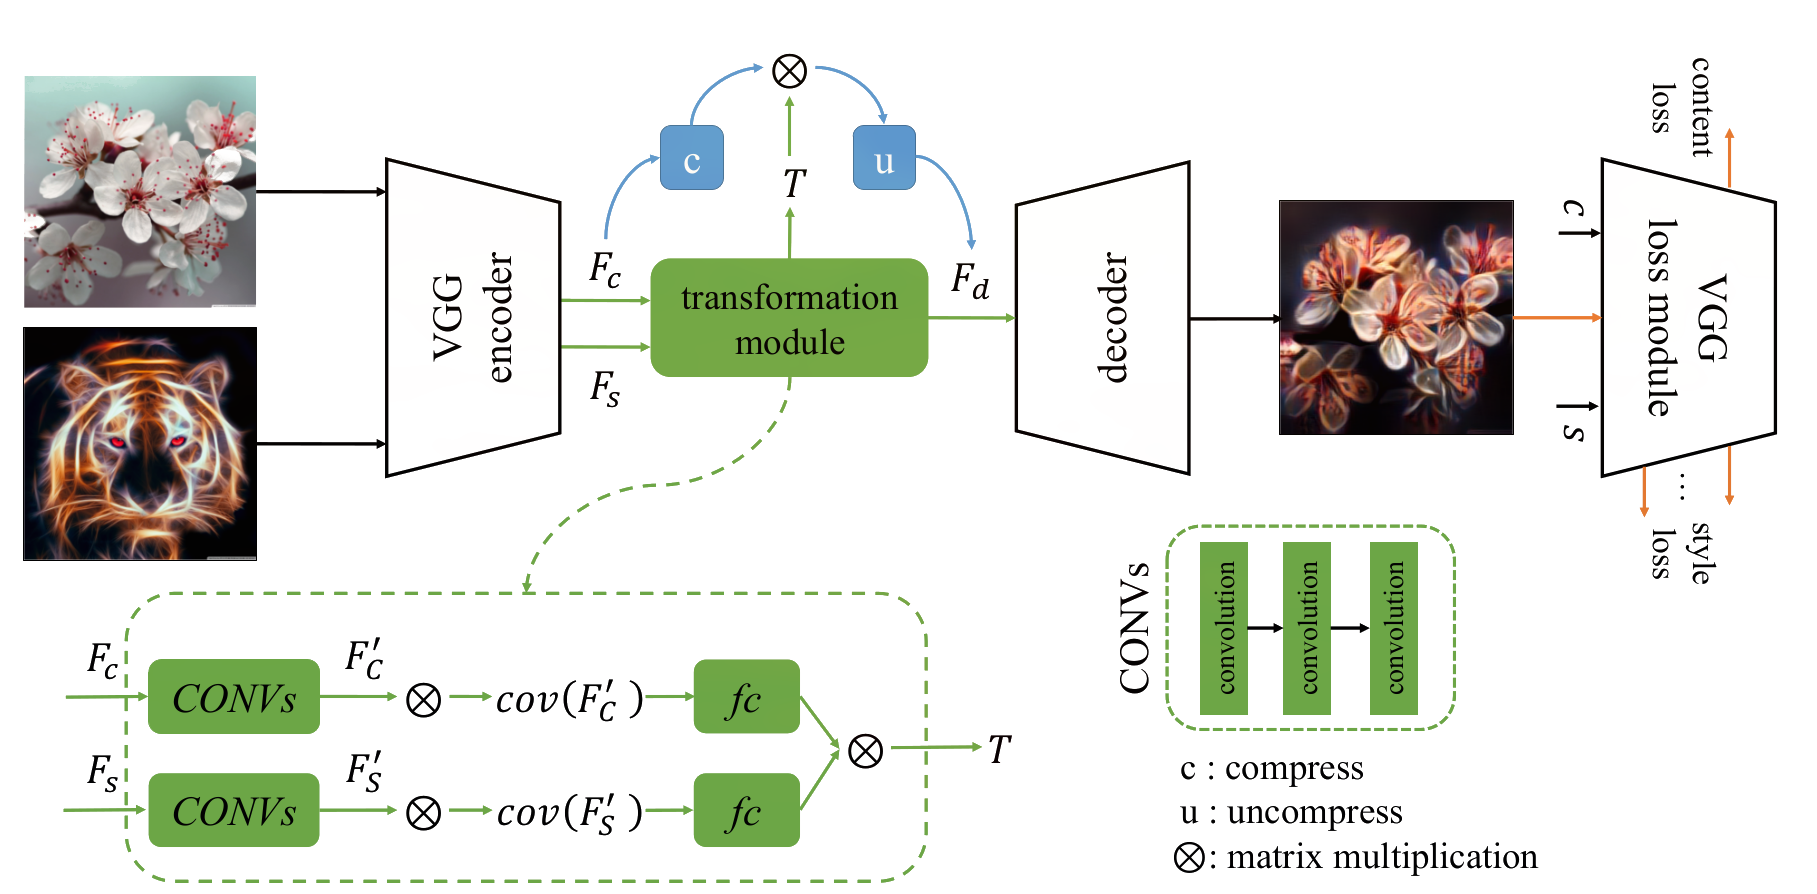
\includegraphics[scale=0.25]{overall_network.png}
        \caption{Overview of the network architecture}
        \label{fig:overall_network}
    \end{figure}
    
    
    \subsubsection{Encoder-decoder}
    Both encoder and decoder are based on first layers of VGG-like [\cite{vgg}]
    network. VGG is a family of fully convolutional neural networks developed 
    specifically for computer vision task. Full VGG network consists of
    stacked Conv layers with ReLU activation function, interleaved with pooling
    layers performing downsampling, ending with couple of fully
    connected layers and Softmax layer. Such architecture allows for image classification.
    To adapt it for other computer vision tasks like segmentation, object detection,
    tracking, domain adaptation or style transfer, the non-convolutional part
    of network needs to be removed. Depending on task's complexity, desired
    latency and available hardware, vgg-like networks of varying depth can be 
    constructed by simply removing consequent top layers of the network.
    The architecture used by \cite{Li2018} and our pruned version are 
    outlined in table \ref{table:vgg}. 
    
    \begin{table}
    \begin{center}
        \begin{tabular}{|c|c|}
        \hline
         \cite{Li2018} & Our \\
        \hline
          \multicolumn{2}{|c|}{Pointwise Conv(3, 3)} \\
          \hline
          CReLU(3, 64)  & CReLU(3, 16)  \\
          \hline
          CReLU(64, 64) & CReLU(16, 16)  \\
          \hline
          \multicolumn{2}{|c|}{Max Pool x2}      \\
          \hline
          CReLU(64, 128)  & CReLU(16, 32) \\
          \hline
          CReLU(128, 128)  & CReLU(32, 32)\\
          \hline
          \multicolumn{2}{|c|}{Max Pool x2}    \\
          \hline
          CReLU(128, 256) & CReLU(32, 64)\\
          \hline
          CReLU(256, 128) & CReLU(64, 32)\\
          \hline
          \multicolumn{2}{|c|}{Upsample Nearest x2}\\
          \hline
          CReLU(128, 128) & CReLU(32, 32)\\
          \hline
          CReLU(128, 64) & CReLU(32, 16)\\
          \hline
          \multicolumn{2}{|c|}{Upsample Nearest x2}\\
          \hline
          CReLU(64, 64) & CReLU(16, 16) \\
          \hline
          CReLU(64,3) & CReLU(16, 3)\\
          \hline
        \end{tabular}
            \end{center}
        \caption{Encoder-decoder architecture before and after filter pruning.
        The first Conv layer is pointwise convolution with 1x1 kernel, 
        unitary stride, without padding. It has 3 input and 3 output channels.
        \textit{CReLU(a,b)} is Conv layer with \textit{a} input channels and 
        \textit{b} output channels followed by ReLU activation. All of 
        \textit{CReLU}s have 3x3 kernels, unitary stride and and single pixel
        of padding on each of 4 sides. Downsampling and upsampling
        is done with 2x2 kernels and stride 2.
        }
        \label{table:vgg}
    \end{table}
    
    They differ in two aspects:
    \begin{itemize}
        \item \textbf{Padding} - \cite{Li2018} use reflection padding. In many
        models used for style transfer, use of zero padding degrades network's
        performance around the input's edges[\cite{johnson2016perceptual}], exhibiting as
        vanishing of style or artifacts (see figure \ref{fig:edges}).
        In such situation adding reflection padding fixes the issue. We replace
        reflection padding with zero padding, because the former one is not 
        implemented within TensorRT used for additional inference speedup
        (see \ref{trt_chapter}). Fortunately we don't observe described problem
        in our model.
        \begin{figure}[h!]
            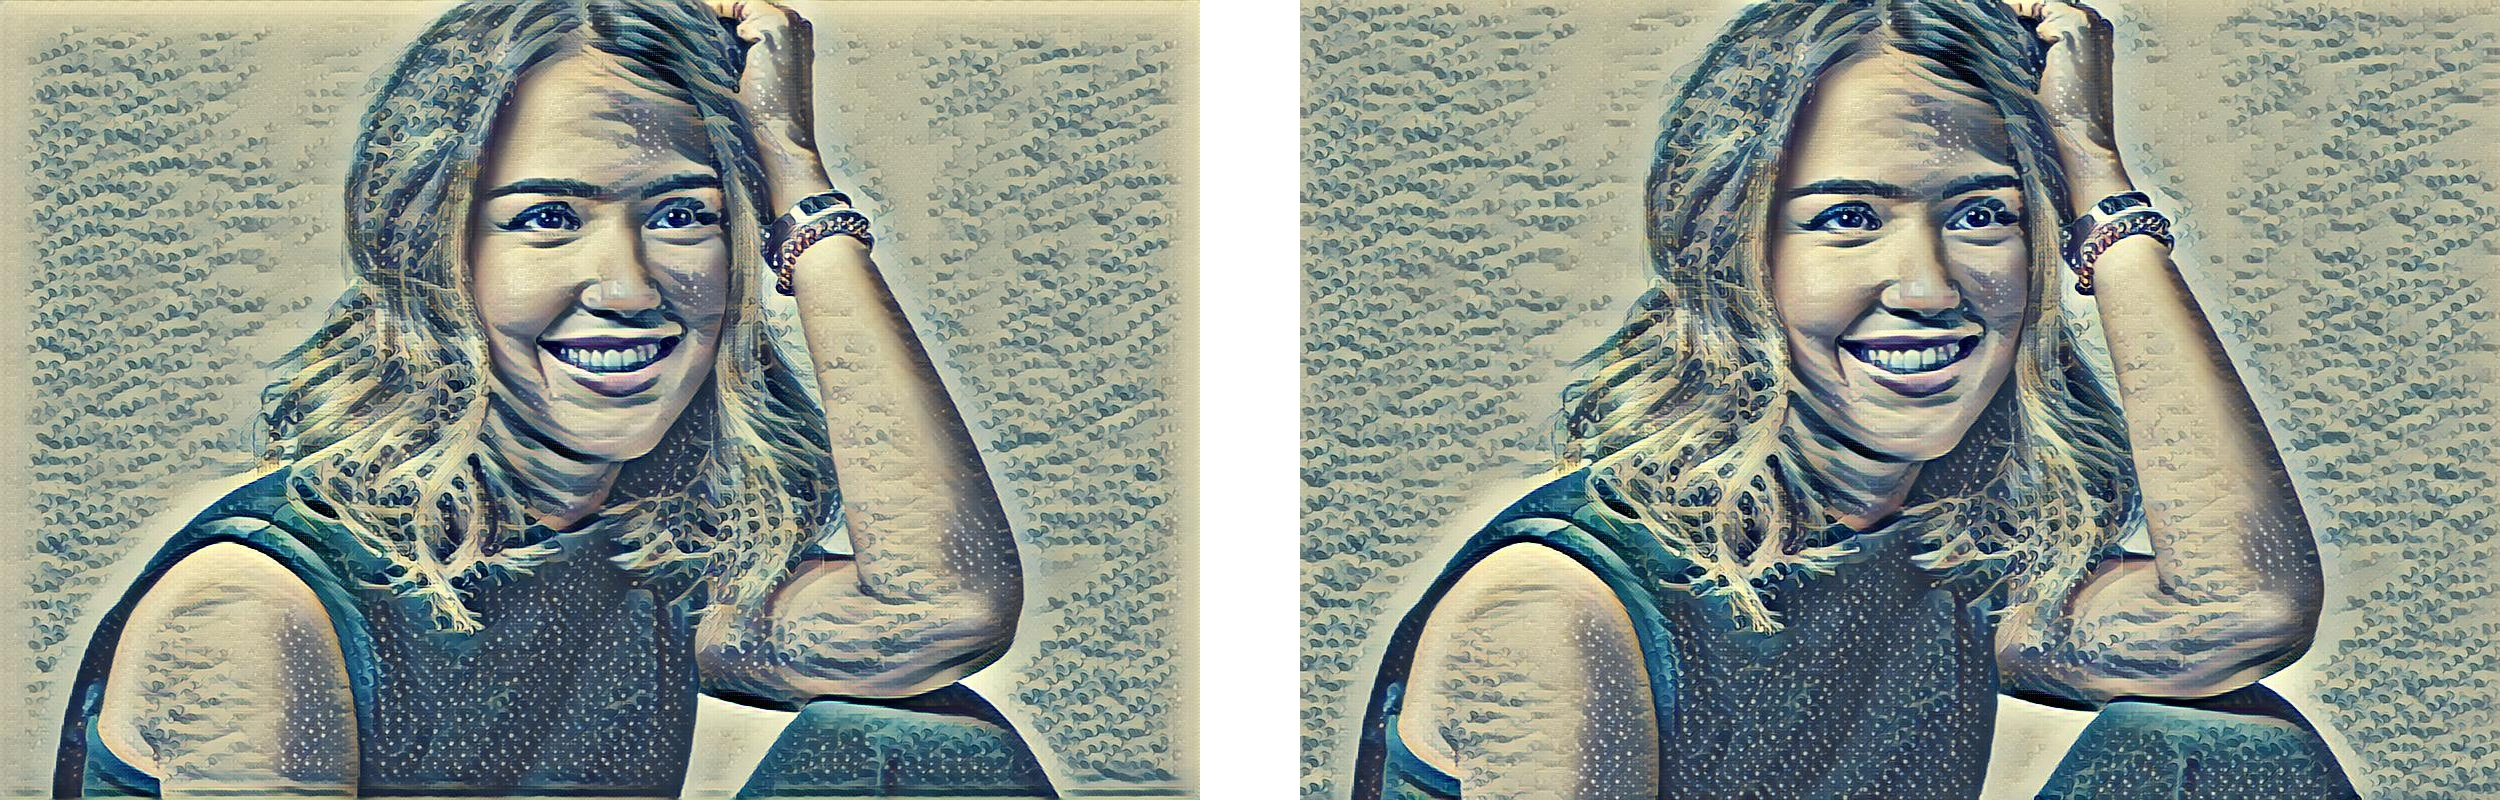
\includegraphics[scale=0.17]{edges.jpg}
            \caption{Result of zero padding (left) and reflection padding (right)
                in \cite{johnson2016perceptual}. Style visibly diminishes around
                the edges in the left image.
            }
            \label{fig:edges}
        \end{figure}
        \item \textbf{Width} of Conv layers. In order to reduce inferencetime ,
        we prune encoder and decoder 
        to only contain $25\%$ of feature maps from the original architecture.
        This provides 
        \kamil{Measure the speedups across couple GPUs 
            (and maybe CPUs)}             
        %TODO
        X-times speedup on NVIDIA GTX 960 GPU inference server is ran on
        [\kamil{refer to speedup table}]
        
    \end{itemize}


    \subsection{Transformation module}

\subsection{Pruning}
    \textbf{Filter pruning} 
    \textbf{Pruning schedule, datasets} 



\biblio % Needed for referencing to working when compiling individual subfiles - Do not remove
\end{document}
